\chapter{Scrum overview}
The concept of agile development was proposed in 2001. Agile Manifesto was elaborated by 17 developers, the purpose of it was to gather all important rules how to properly produce a good quality product:

"We are uncovering better ways of developing
software by doing it and helping others do it.
Through this work we have come to value:

Individuals and interactions over processes and tools \hfill \break
Working software over comprehensive documentation \hfill \break
Customer collaboration over contract negotiation \hfill \break
Responding to change over following a plan \hfill \break

That is, while there is value in the items on
the right, we value the items on the left more." \cite{AgileManifesto}

The Agile Manifesto is based on following twelve principles:

\begin{enumerate}
    \item Our highest priority is to satisfy the customer
through early and continuous delivery
of valuable software.
\item Welcome changing requirements, even late in 
development. Agile processes harness change for 
the customer's competitive advantage.
\item Deliver working software frequently, from a 
couple of weeks to a couple of months, with a 
preference to the shorter timescale.
\item Business people and developers must work 
together daily throughout the project.
\item Build projects around motivated individuals. 
Give them the environment and support they need, 
and trust them to get the job done.
\item The most efficient and effective method of 
conveying information to and within a development 
team is face-to-face conversation.
\item Working software is the primary measure of progress.
\item Agile processes promote sustainable development. 
The sponsors, developers, and users should be able 
to maintain a constant pace indefinitely.
\item Continuous attention to technical excellence 
and good design enhances agility.
\item Simplicity--the art of maximizing the amount 
of work not done--is essential.
\item The best architectures, requirements, and designs 
emerge from self-organizing teams.
\item At regular intervals, the team reflects on how 
to become more effective, then tunes and adjusts 
its behavior accordingly.\cite{AgileManifesto}
\end{enumerate} 

Scrum is the most popular agile methodology for developing products and services \cite{ArticleStateOfAgile}. The \autoref{fig:agileDiagram} shows, in a simplified way, how agile development works \cite{ScrumBook}. The main rule in development using Scrum methodology is that after each iteration (2-4 weeks of implementing planned features) the customer is able to get a usable product. The principle artifact in Scrum is product backlog, which is a list of features based on customer requirements, it should be prioritized from the most important functions to "nice to have" features or just less urgent. The backlog contains user stories, which is a form of expressing business requirement in Scrum, it is created in a way that can be understandable for both sides, business and development. There are a few templates with different structure, but the most popular and commonly used is:

\begin{enumerate}
    \item Basic User Story structure \cite{ScrumBook}
    \begin{enumerate}
        \item As <who, a role in system>, I want <what, a need> so that <benefit, goal> e.g.:
            \begin{enumerate}
                \item As \textit{a company owner}, I want \textit{the company logo to be visible on the welcome page} so that \textit{customers are able to see it}.
            \end{enumerate}
    \end{enumerate}
    \item Mike Cohn's User Story Structure \cite{MikeCohnUS}
    \begin{enumerate}
        \item As <a role>, I want <goal/desire> e.g.:
        \begin{enumerate}
            \item As a \textit{user}, I want \textit{the company logo to be visible on the welcome page}.
        \end{enumerate}
    \end{enumerate}
    \item Chriss Matts's User Story Structure \cite{AntonyMarcanoUS}
    \begin{enumerate}
        \item In order to <receive benefit> as a <role>, I want <goal/desire>
        \begin{enumerate}
            \item In order to \textit{increase the number of sales of our print consumables} as a \textit{marketing manager}, I want \textit{customers to register their e-mail addresses}.
        \end{enumerate}
    \end{enumerate}
\end{enumerate}

A user story is created to store it in Product Backlog and in the future divide it to tasks, but in order to do it developers should know the requirements, so the main purpose of user story is to start conversation, it is a catalyst to talk about requirements.

\begin{figure}[h]
\caption{Agile development overview \cite{ScrumBook}}
\label{fig:agileDiagram}
\centering
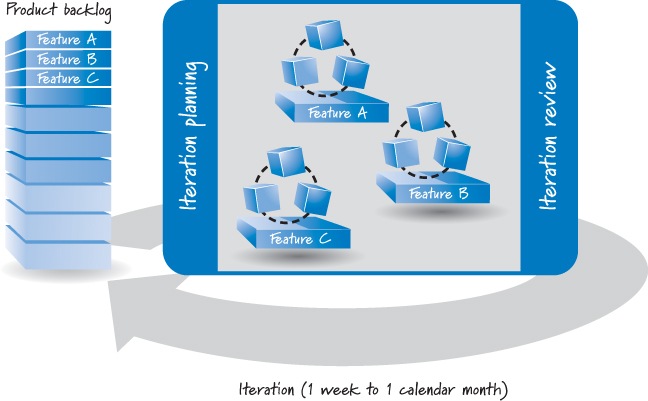
\includegraphics[width=1\textwidth]{img/agileDiagram}
\end{figure}

\section{Scrum in theory}
In this section we will focus on scrum in theory, how it works, what are the required elements - who is required and what meetings. Often scrum in theory differs from scrum in practice and it is said that Scrum is just a tool and it should adjust to the team, not the other way.
\subsection{Process phases}
Scrum is a methodology based on incremental and iterative model of product development cycle as showed on \autoref{fig:agileMethodology}.

\begin{figure}[h]
\caption{ Scrum cycle development}
\label{fig:agileMethodology}
\centering
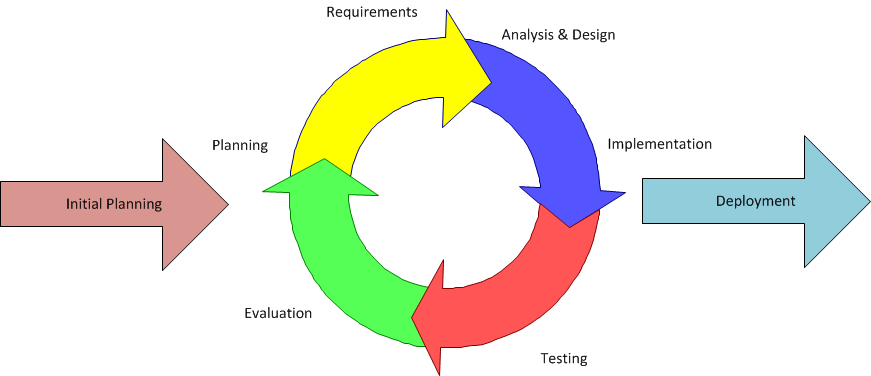
\includegraphics[width=1\textwidth]{img/iterativeScrum}
\end{figure}

The incremental-iterative model is divided into stages, one whole cycle is called sprint, it is suggested that each sprint should be 2-4 weeks long. Every cycle contains planning, gathering requirements and deciding, what and how should be done, analysis and design, implementing what was planned on the particular iteration, in this moment of cycle we have two paths, we can decide to deploy our product if it is done or continue to next stage which is testing. The last element of the cycle is evaluation, if everything what was planned was actually implemented. The cycle is actually straight-forward and is very effective \cite{ScrumBook}.

\subsection{Roles in scrum}
Scrum has determined each team member included in the project a particular role \autoref{fig:rolesScrum}, each role has it's own responsibilities.

\begin{figure}[h]
\caption{Roles in scrum \cite{ScrumBook}}
\label{fig:rolesScrum}
\centering
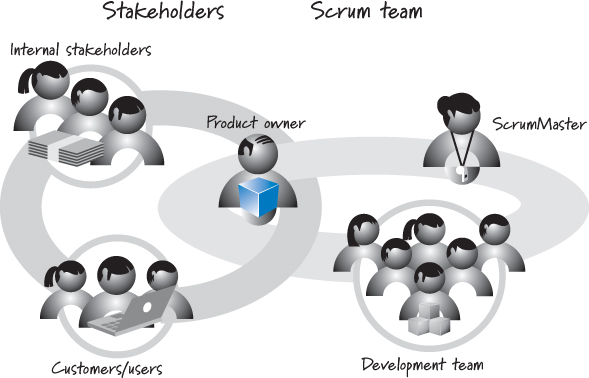
\includegraphics[width=0.75\textwidth]{img/roles}
\end{figure}

Product owner is a person that need to look in at least two directions simultaneously \cite{ScrumBook}. This role is responsible for communication between stakeholders and the scrum team. The principle obligations are shown in the \autoref{fig:prodOwnerRes}.

\begin{figure}[h]
\caption{Product owner responsibilities \cite{ScrumBook}}
\label{fig:prodOwnerRes}
\centering
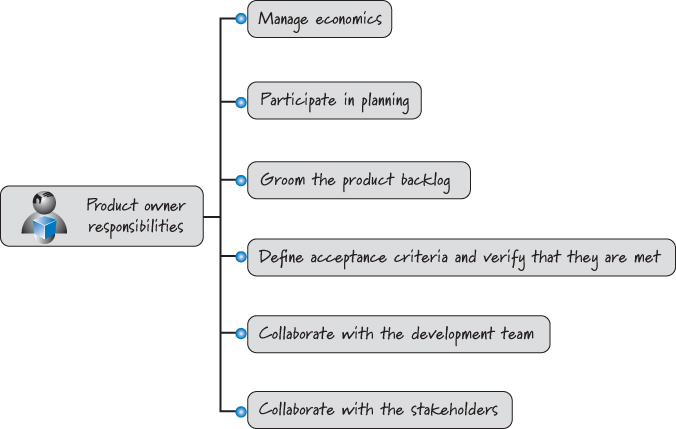
\includegraphics[width=0.75\textwidth]{img/prodRes}
\end{figure}

Product owner represents scrum team outside and is responsible for product development, decides which feature should be included in a particular sprint, adds user stories and features to the backlog, defines acceptance criteria and verifies whether they are full filled after the sprint. 

Another important person in Scrum Team is Scrum Master, whose responsibility is illustrated on \autoref{fig:masterRes}. Mainly his role is to superintend the process and help development team to adapt to the agile methodology. This role is responsible mainly for removing impediments that inhibit team's productivity, protects team from outside interference so that they can remain focused on delivering good quality business value every sprint, servant leader of the Scrum team and team's process authority \cite{ScrumBook}.

\begin{figure}[h]
\caption{Scrum master responsibilities \cite{ScrumBook}}
\label{fig:masterRes}
\centering
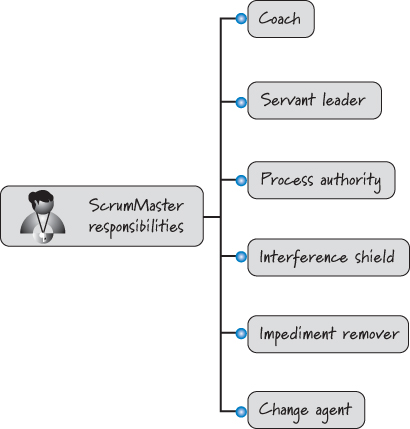
\includegraphics[width=0.5\textwidth]{img/masterRes}
\end{figure}

The last, but without which there would be no product and which is essential, is development team, also called delivery team, design-build-test team or just team. Types of jobs in a development team for example are: architect, programmer, tester, database administrator, user interface designer and many more. Development team is responsible for product implementation, testing, integration and design. The team should include people of various specializations and skills, who can fulfill project requirements. Delivery team is obliged to perform sprint execution, which means performing actions that will result with a ready functionality. Each member of the team is expected to participate in scrum meeting such as described in \autoref{chap:meetingsOverview}. On this group this work will be mainly focused on \cite{ScrumBook}.

\begin{figure}[h]
\caption{Development Team responsibilities \cite{ScrumBook}}
\label{fig:devtRes}
\centering
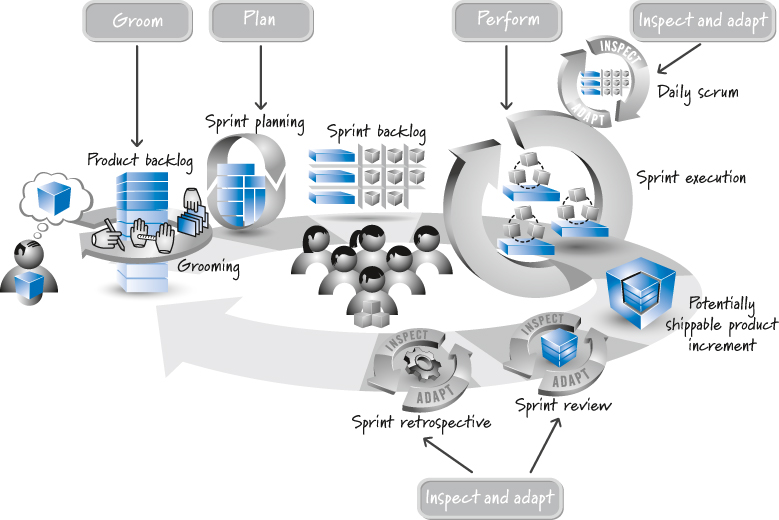
\includegraphics[width=1\textwidth]{img/developmentRes}
\end{figure}

\subsection{Meetings overview}
\label{chap:meetingsOverview}

A product development is composed of multiple sprints, which can last 2-4 weeks \cite{ScrumBook} and each iteration should deliver a usable product to a customer, which does not mean ready or fully functional implementation, just a product that can be potentially shippable. As presented on \autoref{fig:meetingsScrum}, before sprint execution there should be a Backlog Grooming meeting, each iteration starts with Sprint planning and ends with Sprint Review and Retrospective, what is more every day begins with Daily Scrum. The next sections will describe all the meetings separately \cite{ScrumBook}. 

\begin{figure}[h]
\caption{Scrum meetings and process}
\label{fig:meetingsScrum}
\centering
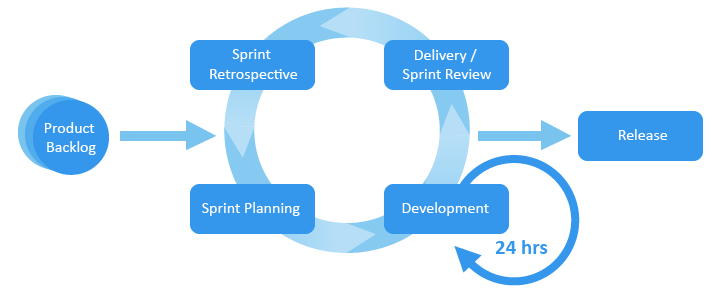
\includegraphics[width=1\textwidth]{img/agile-graphic}
\end{figure}

This Backlog grooming meeting is focused on maintaining the product backlog, it should be executed before next sprint planning. The main aim of this meeting is to \cite{ScrumBook2}:

\begin{itemize}
    \item remove user stories that are no longer relevant,
    \item creating new user stories in response to newly discovered needs,
    \item prioritizing the user stories, 
    \item assigning or correcting estimates to user stories,
    \item splitting user stories which are high priority but too big to fit in an upcoming iteration.
\end{itemize} 

On the Backlog Grooming it is mandatory that the Product Owner is present, Developments' Team and Scrum Masters' presence is optional \cite{ScrumBook}.

The Sprint Planning is a meeting on which Product Owner shares initial sprint goal and answers questions regarding product backlog items. The initial requirements should be accomplished in order to start the meeting \cite{IntroToScrumBook}:
\begin{enumerate}
    \item Prioritized backlog after backlog grooming.
    \item The highest-priority stories should be estimated.
    \item Prepared definition of done.
    \item The capacity of the team should be known, for example the team has a meeting outside working place that might affect the sprint, this should be included in the capacity field.
\end{enumerate}
Two distinct objectives might be retrieved from the Sprint planning. Firstly, we must ensure that each team member understands what is expected to do in the particular user story and secondly divide user stories into tasks and determine what can they deliver and makes a realistic commitment. Each team member might select one of the tasks, which is willing to own and complete, but it is not a required action, which must be performed. Thereafter, the team estimates, taking all the factors into the consideration, the risk, developers experience, the difficulty of the task and estimate in hours how long it might take to complete a task. From the Sprint planning we have two primary outputs, first is the goal of the iteration, which means, what users stories should be delivered, second is the sprint backlog with list of created tasks \cite{ScrumBook, IntroToScrumBook}. 

\begin{figure}[h]
\caption{Scrum One-part sprint-planning approach \cite{ScrumBook}}
\label{fig:planningDiagram}
\centering
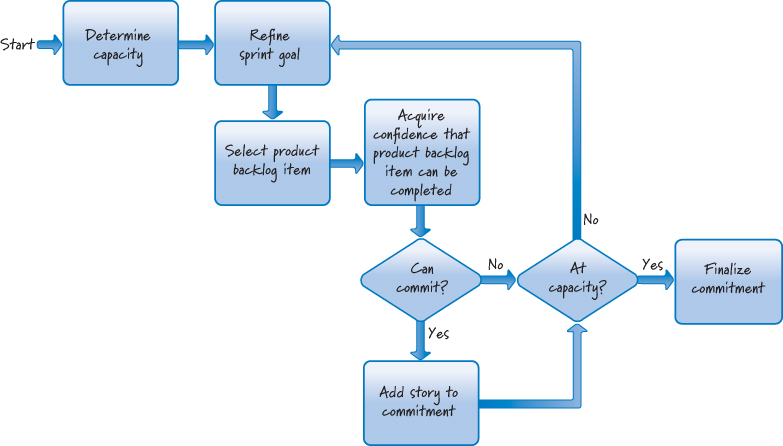
\includegraphics[width=1\textwidth]{img/sprintPlanning}
\end{figure}

The Review is a meeting in Scrum which takes place at the end of an iteration. The product owner, scrum master and development team should be present, on the list of invited people might customers and managers may be included. The review meeting is a demo of a product that has been delivered after a sprint and also a chance for the customers to provide feedback. Quoting the agile manifesto "Working software is the primary measure of progress." and "Welcome changing requirements, even late in development. Agile processes harness change for the customer's competitive advantage." those rules are fulfilled thanks to the review meeting \cite{DotNetScrumBook}.

The Daily Stand-ups is a short meeting which is held every day during the sprint and its purpose is to discuss issues that are preventing work from being done and how is the work progress. The Daily Stand-ups are time boxed to no longer than 15 minutes and the participants are obliged to stand. The team members stand in the circle and and answer the following questions \cite{DotNetScrumBook}:
\begin{enumerate}
    \item What have you done since yesterday?
    \item What are you planning to do today?
    \item Do you have any problems preventing you from accomplishing your goal? What progress has been made on existing impediments? Can the blockage be removed or must it be escalated?
\end{enumerate}

It is indicated that in order to keep the meeting short, the major issues which were discovered during the Daily Stand-up will be discussed afterwards \cite{DotNetScrumBook}.

The Retrospective meeting takes place at the end of the meeting and is strictly focused on reflection of team members on the sprint that has passed. The encounter provides the participants a chance to congratulate each other on the things that succeeded and discuss once that went wrong \cite{DotNetScrumBook}. The purpose of the retrospective was summarized by Norm Kerth, by quoting a fragment from "Winnie the Pooh" \cite{ScrumBook}:
\begin{displayquote}
Here is Edward Bear, coming downstairs now, bump, bump, bump, bump, on the back of his head, behind Christopher Robin. It is, as far as he knows, the only way of coming downstairs, but sometimes he feels that there is another way, if only he could stop bumping for a moment and think of it.
\end{displayquote}

The Sprint Retrospective allows the participants to stop bumping and have a moment to think. The target is to examine what is happening in the team, analyze the way the team is working, identify the problems and ways to improve. The areas that the team should focus on and which are up for discussion are processes, practices, communication, environment, artifacts, tools, internal and external issues within the project and the development group \cite{ScrumBook}.

It is said that the Sprint Retrospective is one of the most important and least appreciated practices in the Scrum and this is because there are people who think that it takes time away from doing "real things" such as developing, testing, designing. Its importance comes from fact that using this approach the team members are able to customize scrum to theirs needs and it is a crucial contributor, as written in Agile Manifesto \cite{AgileManifesto}, to continuous improvement \cite{ScrumBook}.

\section{Scrum in practice}

In order to evaluate how Scrum appears in practice, the best strategy is to ask the people who deal with it every day e.g. developers. The focus group is a form of research which includes people discussing their opinions and attitudes about a particular subject. The focus group has been created to retrieve the opinions about Scrum in practice. They were asked a set of eight questions listed below:
\begin{enumerate}
    \item Engagement questions:
    \begin{enumerate}
        \item How and from whom did you first learn about the Scrum framework?
    \end{enumerate}
    \item Exploration questions:
    \begin{enumerate}
        \item What were your biggest pitfalls/impediments in the case of Agile Methodologies in your career?
        \item What are the pros and cons of Scrum?
        \item What Scrum practices are you following and which are you not? Why? (Meetings, Sprints, Roles, Iterative and incremental practices, Product Backlog, Sprint Backlog)
        \item Which meeting do you think is useful and which not? Why?
        \item Which Scrum role do you think is useful and which not? Why?
        \item If you could change the methodology in your team, what would it be?
    \end{enumerate}
    \item Exit question:
    \begin{enumerate}
        \item Is there anything else you would like to add to the discussion about Scrum?
    \end{enumerate}
\end{enumerate}

The group contained twelve people and the profiles of the developers are presented on the \autoref{tab:profiles}.

\begin{table}[ht!]
\caption{Participants of focus group profiles}
\label{tab:profiles}
\begin{tabularx}{\textwidth}{|X|X|X|}
\hline
\textbf{Role} & \textbf{Experience in IT} & \textbf{Quantity}  \\ \hline
Scrum master & 10 years & 1 \\ \hline
Product Owner & 2 years & 1 \\ \hline
Design Lead & 10 years in development, 1 year as design lead & 1 \\ \hline
Developer & around 2-3 years on average & 7 \\ \hline
Developer & 6 years & 1 \\ \hline
Developer Intern & 6 months & 1 \\ \hline
\end{tabularx}
\end{table}

After the meeting, where the discussion took place, we evaluated the results and they were satisfactory. The goal of the focus group which is "continue the discussion until no more new ideas appear" had been achieved.

In the first question, the warming up and introduction to the subject, most of the participants revealed that they found out and learned scrum at work or university. Two out of twelve participants attended Scrum courses.

On the question "What were your biggest pitfalls/impediments in the case of Agile Methodologies in your career?" the participants retrieved five main ideas:
\begin{enumerate}
    \item It is hard to work in a big team with multiple small agile teams, when there are many dependencies between those small teams.
    \item There is a lack of discipline during daily team scrums - short summaries of everyday problems tended to evolve into long discussions.
    \item Many people have different views of what Agile is, and because of this many companies interpret what Agile must consist of. 
    \item The inability for a company to change their interpretation of Agile to better suit their business.
    \item Bad interpretation of the Scrum leads to chaotic work.
\end{enumerate}

Participants' opinions on the pros of the Scurm are as follows:
\begin{enumerate}
    \item Regular meetings keep teams focused.
    \item Scrum is easy to manage and creates room for improvement. 
    \item Scrum efficiently organizes the work in development teams and clearly separates "What we do?" from "How will we do it?".
    \item Operating on timeboxing, which is the time taken for a task to be completed.
    \item Builds good habits like for example, sprints - work in an equal and repeatable manner in the case of time segments.
    \item Predictable methodology - provides metrics that can measure the tempo of the work and capacity.
    \item Developers like to focus on work without major interruptions.
    \item Continuous development thanks to the retrospective meetings.
    \item Flexible in case of changes to the market and no need to prepare a documentation before the project starts.
    \item Scrum is flexible, allows teams to self-organize themselves.
    \item Fast iterations and feedback.
    \item Scrum meetings are helpful in terms of relations between people.
    \item One of the least restrictive methodologies and due to that, it is a appropriate choice to chose Scrum.
    \item Spreading the knowledge about current tasks among the entire project group - everyone is better oriented about all current tasks in the team. Technical knowledge is better spread among team members - good way to known if someone has previously dealt with similar issues.
    \item Large projects are divided into easily manageable sprints.
    \item Works well for fast-moving development projects.
    \item Scrum, being agile, allows to retrieve feedback from customers and stakeholders.
\end{enumerate}

And regarding the answer on the second part of the third question - the cons are as follows:

\begin{enumerate}
    \item In big projects, there is no need to plan everything straight away.
    \item Teams takes ownership, so lazy teams means bad results.
    \item It is hard to convince the client to collaborate and participate in the project. They are used to work that is based on a specific model in which they are expecting the work to be done in a defined period of time after the payment.
    \item It is hard to understand the simple rules of Scrum for the customer.
    \item It is hard to accept the symbiosis of the Development Team and the Product Owner. Unfortunately, very often the business is separated from the developers and they come up with ideas that are not useful, but the developers are forced to implement it. 
    \item There is no good place for unexpected bug fixing during sprint.
    \item Most of the people do not understand Scrum and claim that they are using it.
    \item The duration of the meetings should be decreased.
    \item Time overspent on daily statuses reports and planning.
    \item Most of the time spent on daily scrums brings little value - it seems like it involves just listening to the team members' thoughts and problems without a perspective to actually help people out.
    \item Scrum often leads to scope creep, due to the lack of a definite end-date.
    \item Adopting the Scrum framework in large teams is challenging.
    \item Based on external research, the best quantity of team members is a team of seven as people then feel like a family.
\end{enumerate}

The pros of the Scrum are extending the cons which is satisfying. In the group there were Scrum "lovers" and Scrum "haters" so it is a success that the number of positive aspects of Scrum was larger than the negative.

The fourth question was about Scrum practices used in the participants' teams. A few of them did not see the point of following any of the meetings, besides Daily Stand-ups and claimed that their team does not do that. A few of the attendants of the focus group did not understand the meaning of these practices in scrum and they felt like they were forced to do them, because of the place they work at. The majority understands and thinks that most of the Scrum Practices are useful and helpful for the project:
\begin{enumerate}
    \item Daily Stand-ups in the same place and at the same time.
    \item The best quantity of team members is a team of seven, based on the external researches, as people then feel like a family.
    \item Retrospective is a key to success as it helps to develop the project and the team.
    \item Backlog and Sprint Backlog are crucial for development, but unfortunately very often there is too little time for that.
\end{enumerate}

In case of the usefulness of the meetings, the common opinion was that meetings that require discussion over matters that share ownership are important. If an issue has one owner, there should not be a meeting unless completely necessary. The majority of the participants did not see the point of attending all the meetings as they found that only Sprint Planning and the Sprint Stand-ups were useful. Only three out of twelve people agreed on the importance of all the meetings.

The sixth question was about the usefulness of the roles in Scrum. The participants agreed that they are all useful if done correctly and fit the business processes of the company.

The last question of exploration questions was about changing the methodology in the team. Only one of the participants said they would change the methodology to Kanban. The rest of the research attendants, who were previously able to retrieve a number of cons regarding the Scrum, said they would stay with the Scrum as they believed it is the best methodology.

The exit question brought a new topic to the table. The participants agreed that they in general do not understand Scrum. It has been suggested that each member of the Scrum team should read a Scrum Guide a few times and think about what "timebox", "definition of done" and "commitment to deliver a task at the end of the sprint" means to them. What is more, the most common Scrum mistakes were retrieved:
\begin{enumerate}
    \item Forgetting about Scrum Retrospective meetings.
    \item Not following the "definition of done" while ending a task.
    \item Not considering the capacity of the team during a Scrum Planning meeting.
    \item The Product Owner tells the team how to implement a feature.
    \item The Development Team does not provide technical feedback to the Product Owner.
    \item The Development Team does not perform Scrum Daily Stand-ups.
    \item During the Scrum Daily Stand-up, the participants would talk about how they implemented a task instead of what they did and what they intend to do.
    \item The Scrum Review meeting is being treated as an acceptance meeting, while the tasks and user stories have to be closed before the meeting.
\end{enumerate}

To conclude, very often the team members using the Scrum methodology do not understand the purpose of this methodology. A requirement in every company should be a good understanding of the methodology that they are using. The organisation should provide their employees with adequate courses and coaches that will tell them how Scrum works and what its aim is. Moreover, Scrum is very often underestimated, despite it being the most popular used approach in case of developing software.

\section{Conclusions}

Nowadays Scrum is the most popular agile methodology for developing products and services \cite{ArticleStateOfAgile}, but usually is not implemented as designed. People tend to change the Scrum in order to adjust it for their purpose. For example, following only two meetings, because they do not see the purpose of the other Scrum meetings. Another discovered issue is that team members do not understand Scrum, which creates a major aversion to it. The developers feel that the time spent on the meetings is a waste of time and they like to focus on work without major interruptions. Most of the participants of the focus group claimed that if they could, they would only attend on Scrum Planning meeting and Daily Stand-Ups meeting, but usually they are forced to participate in all of them. The latter creates another issue, forcing team members to attend a meeting that they do not understand may result in aversion to it or in some cases permanent removal of the meeting.

The most underestimated meeting is the Scrum Retrospective meeting, because it mainly focuses on the improvement and on the people. During the focus group we learned that some of the participants know the Retrospective only in theory, but they never experienced it in practice. Moreover, based on the focus group research the aversion to Scrum Retrospective meeting is common, even the participants who experienced the Retrospective meeting feel that it is a time consuming and useless meeting. The lack of understanding and implementing Retrospective not as designed is the reason of the aversion and the cause of the underestimation of the Retrospective meeting. Thanks to the Retrospective meeting we are able to achieve a continuous development in terms of the project and the relations between the team members. 

It is impossible to create a perfect methodology and Scrum is not a perfect solution, but it solves plenty of issues, helps the team to self-organize and allows to efficiently develop a product.
